% Valentino Vranic
% Metody inzinierskej prace 2012/13

\documentclass{beamer}

%\usetheme{Warsaw}
%\usetheme{Antibes}
\usetheme{Berkeley}
%\usetheme{Goettingen}

%\usecolortheme{seahorse}
\usecolortheme{dolphin}
%\usecolortheme{rose}
% http://deic.uab.es/~iblanes/beamer_gallery/index_by_color.html
%\usecolortheme{beaver}

%\useoutertheme[]{sidebar}

\setbeamercovered{transparent}

\usepackage[slovak]{babel}
\usepackage[T1]{fontenc}
\usepackage[utf8]{inputenc}
\usepackage{url}
\usepackage{csvsimple}

\usepackage{listings}

\lstset{language=C++,basicstyle=\fontsize{8}{9.6}\selectfont,showstringspaces=false,columns=fullflexible,identifierstyle=\ttfamily,keywordstyle=\bfseries,showstringspaces=false,columns=fullflexible}
%\lstset{language=C,basicstyle=\fontsize{10.5}{12.6}\selectfont,identifierstyle=\ttfamily,keywordstyle=\bfseries,showstringspaces=false,columns=fixed}

\def\BibTeX{\textsc{Bib}\kern-.08em\TeX} 

\newcommand{\footcite}[1]{\footnote{\tiny #1}}
\newcommand{\umlet}{.5}
\newcommand{\emp}[1]{\textit{\alert{#1}}}
\newcommand{\kw}[1]{\mbox{\textbf{#1}}}
\newcommand{\id}[1]{\texttt{#1}}
\newcommand{\stl}{\guillemotleft}
\newcommand{\str}{\guillemotright}

\newcommand{\lsti}{\lstinline[basicstyle=\fontsize{10.5}{12.1}\selectfont]}

\newcommand{\ssection}[1]{
	\section{#1}
	\begin{frame}[fragile=singleslide]\frametitle{}
	\Huge #1
	\end{frame}
}

\newcommand{\ssectionn}[1]{
	\section*{#1}
	\begin{frame}[fragile=singleslide]\frametitle{}
	\Huge #1
	\end{frame}
}

\newenvironment{program}{\begin{beamercolorbox}[rounded=true,shadow=true]{block body}\vspace{-4mm}}{\vspace{-2mm}\end{beamercolorbox}}

\setbeamercolor{fvystup}{fg=white,bg=black}
\newenvironment{vystup}{\begin{beamercolorbox}[rounded=true,shadow=true]{fvystup}}{\end{beamercolorbox}}

\newenvironment{poznamka}{\begin{beamercolorbox}[rounded=true,shadow=false]{block body}}{\end{beamercolorbox}}

\setbeamertemplate{footline}[page number]
{
%\insertpagenumber
%\begin{beamercolorbox}{section in head/foot}
%\vskip2pt\insertnavigation{\paperwidth}\vskip2pt
%\end{beamercolorbox}%
}



\author{Jaroslav Ertl}
%\url{www.fiit.stuba.sk/~vranic}, \url{vranic@fiit.stuba.sk}}
%{\tiny \url{www.fiit.stuba.sk/~vranic}, \url{vranic@fiit.stuba.sk}}
\institute{
       Institute of informatics, information systems and software engineering\\
	Faculty of informatics and information technology\\
	Slovak University of Technology in Bratislava}

\subtitle{\vspace{3mm} Engineering methods 2023/2024}

\title{Examples of search algorithms used in IR
}

\date{\footnotesize 26. november 2023}




\begin{document}

\begin{frame}[fragile=singleslide]
\titlepage
\end{frame}


\begin{frame}[fragile=singleslide]\frametitle{Table of contents}
\tableofcontents
\end{frame}

\section*{Introduction}
\begin{frame}[fragile=singleslide]\frametitle{Introduction}
\begin{itemize}
    \item What is an algorithm
    \item Importance of algorithms
    \item  Different types of algorithms
\end{itemize}

\end{frame}


\section{HITS}
% príkaz \ssection by vytvoril zvláštný slajd s názvom časti - v krátkych prezentáciách to prekáža, lebo oberá o čas

\begin{frame}[fragile=singleslide]\frametitle{Hyperlink-Induced Topic Search(HITS)}
\begin{columns}
    \begin{column}{0.6\textwidth}\begin{itemize}
    \item High-quality pages should link and be linked to by high-quality pages
    \item Score given to a page
    \begin{itemize}
        \item Authority
        \item Hub
    \end{itemize}
    \item Algorithm steps
    \item Problem with bigger networks
\end{itemize}
    \end{column}
    \begin{column}{0.4\textwidth}
      % Image on the right side
      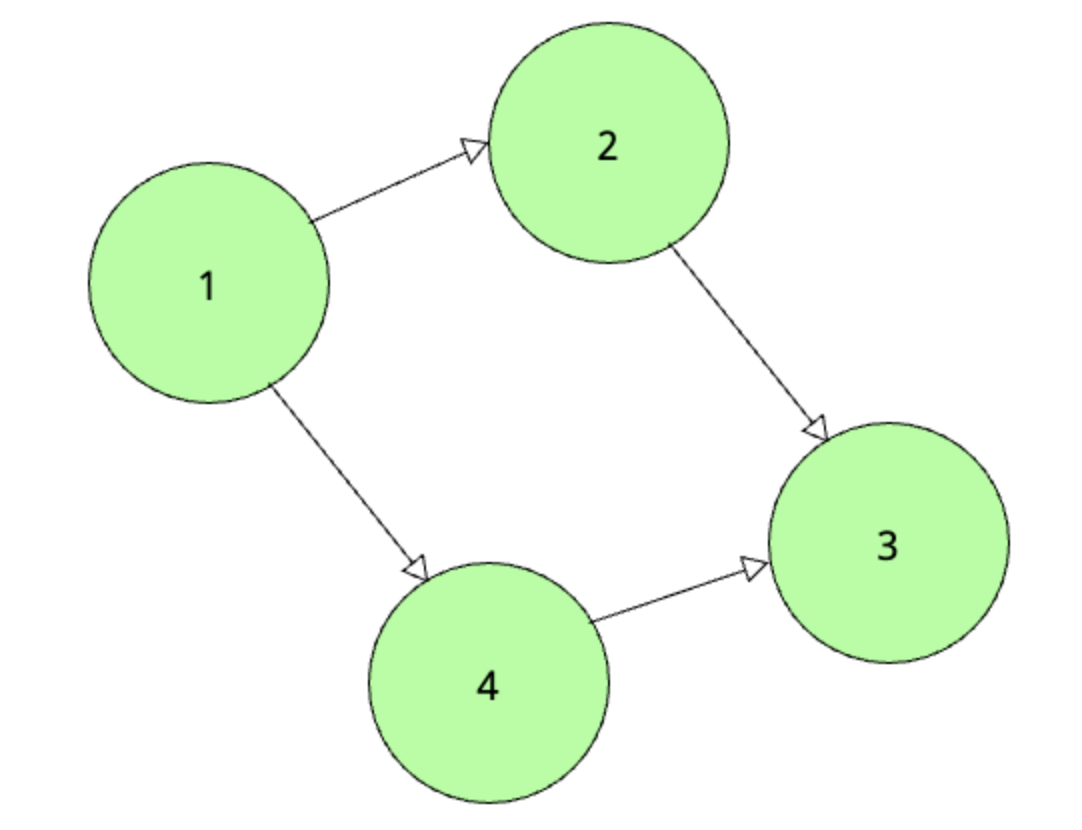
\includegraphics[width=\textwidth]{explanation_HITS.png}
    \end{column}
  \end{columns}
\end{frame}

\section{PageRank}

\begin{frame}[fragile=singleslide]\frametitle{PageRank}
\begin{itemize}
    \item Similar to HITS
    \item PageRank score
    \item Damping factor
    \item Algorithm steps
\end{itemize}
    \begin{poznamka}    
    \[
    PR(p_i) = \frac{1 - d}{N} + d \sum_{p_j \in M_{p_i}} \frac{PR(p_j)}{L(p_j)}\quad \footcite{\url{https://ieeexplore.ieee.org/stamp/stamp.jsp?tp=&arnumber=10210566&isnumber=10005208}} 
    \]
    \end{poznamka}
\end{frame}

\section{Boolean Search}
\begin{frame}[fragile=singleslide]\frametitle{Boolean Search}
\begin{itemize}
    \item Keyword-based
    \item Modifying query with operators - NOT, AND, OR
    \item More operators = less results and more relevant 
    \item Pros
    \begin{itemize}
        \item Eliminate unwanted page fasts
        \item Can be applied to any page
        \item Predictable results
    \end{itemize}
    \item Cons
    \begin{itemize}
        \item Efficiency relies solely on user  
    \end{itemize}
\end{itemize}
\end{frame}


\begin{frame}[fragile=singleslide]\frametitle{Research}
\centering Research with boolean operators done on Google
\begin{figure}[h]
  \centering
  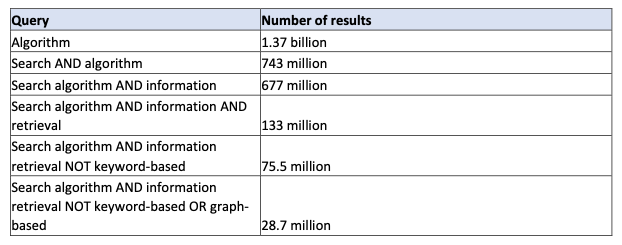
\includegraphics[width=1\textwidth]{BooleanSearch_Table.png}
\end{figure}
\end{frame}
\section{VSM}
\begin{frame}[fragile=singleslide]\frametitle{Vector Space Model}
\begin{itemize}
    \item Page represented as multidimensional vector
    \item Terms and weights reflects the importance in space
    \item Multiple implementations of basic VSM
    \item TF-IDF(Term Frequency- Inverse Document Frequency)
\end{itemize}
\end{frame}



\section*{Summary and upcoming work }
% hviezdička zabezpečí, aby sa táto časť neocitla v prehľade prezentácie - každá prezentácia má zhodnotenie a prehľad by sa tým zbytočne zahlcoval

\begin{frame}[fragile=singleslide]\frametitle{Summary and upcoming work}
\begin{itemize}
    \item Algorithms play crucial role in IR 
    \item An introduction into the world of algorithms
    \item Foundation for next generation algorithms
    \item Finalize the keyword-based algorithms and TF-IDF sections 
\end{itemize}
\end{frame}
\begin{frame}{}
    \centering Thank you for your attention!
\end{frame}


\end{document}




Text \end{document} za príkazom \end{document} LaTeX ignoruje, takže tu môžete odkladať veci (aj celé slajdy), ktoré nechcete vymazať, lebo ich ešte možno budete potrebovať, avšak ich v danom momente nechcete mať v slajdoch.
